%%================================================
%% Appendix J
%%================================================
\chapter[Comparative Performance Evaluation of BLE-Based Indoor Motion Tracking]{\texorpdfstring{ภาคผนวก ญ\\Comparative Performance Evaluation of BLE-Based Indoor Motion Tracking Using Machine Learning and Large Language Models}{Appendix J: Comparative Performance Evaluation of BLE-Based Indoor Motion Tracking Using Machine Learning and Large Language Models}}
\label{app:paperieee_extract}

ภาคผนวกนี้แนบเอกสารเรื่อง \textit{Comparative Performance Evaluation of BLE-Based Indoor Motion Tracking Using Machine Learning and Large Language Models} ฉบับเต็ม ซึ่งใช้เป็นเอกสารประกอบการทดลอง BLE RSSI, KNN, XGBoost และการเปรียบเทียบกับ Large Language Models ในหัวข้อ indoor motion tracking

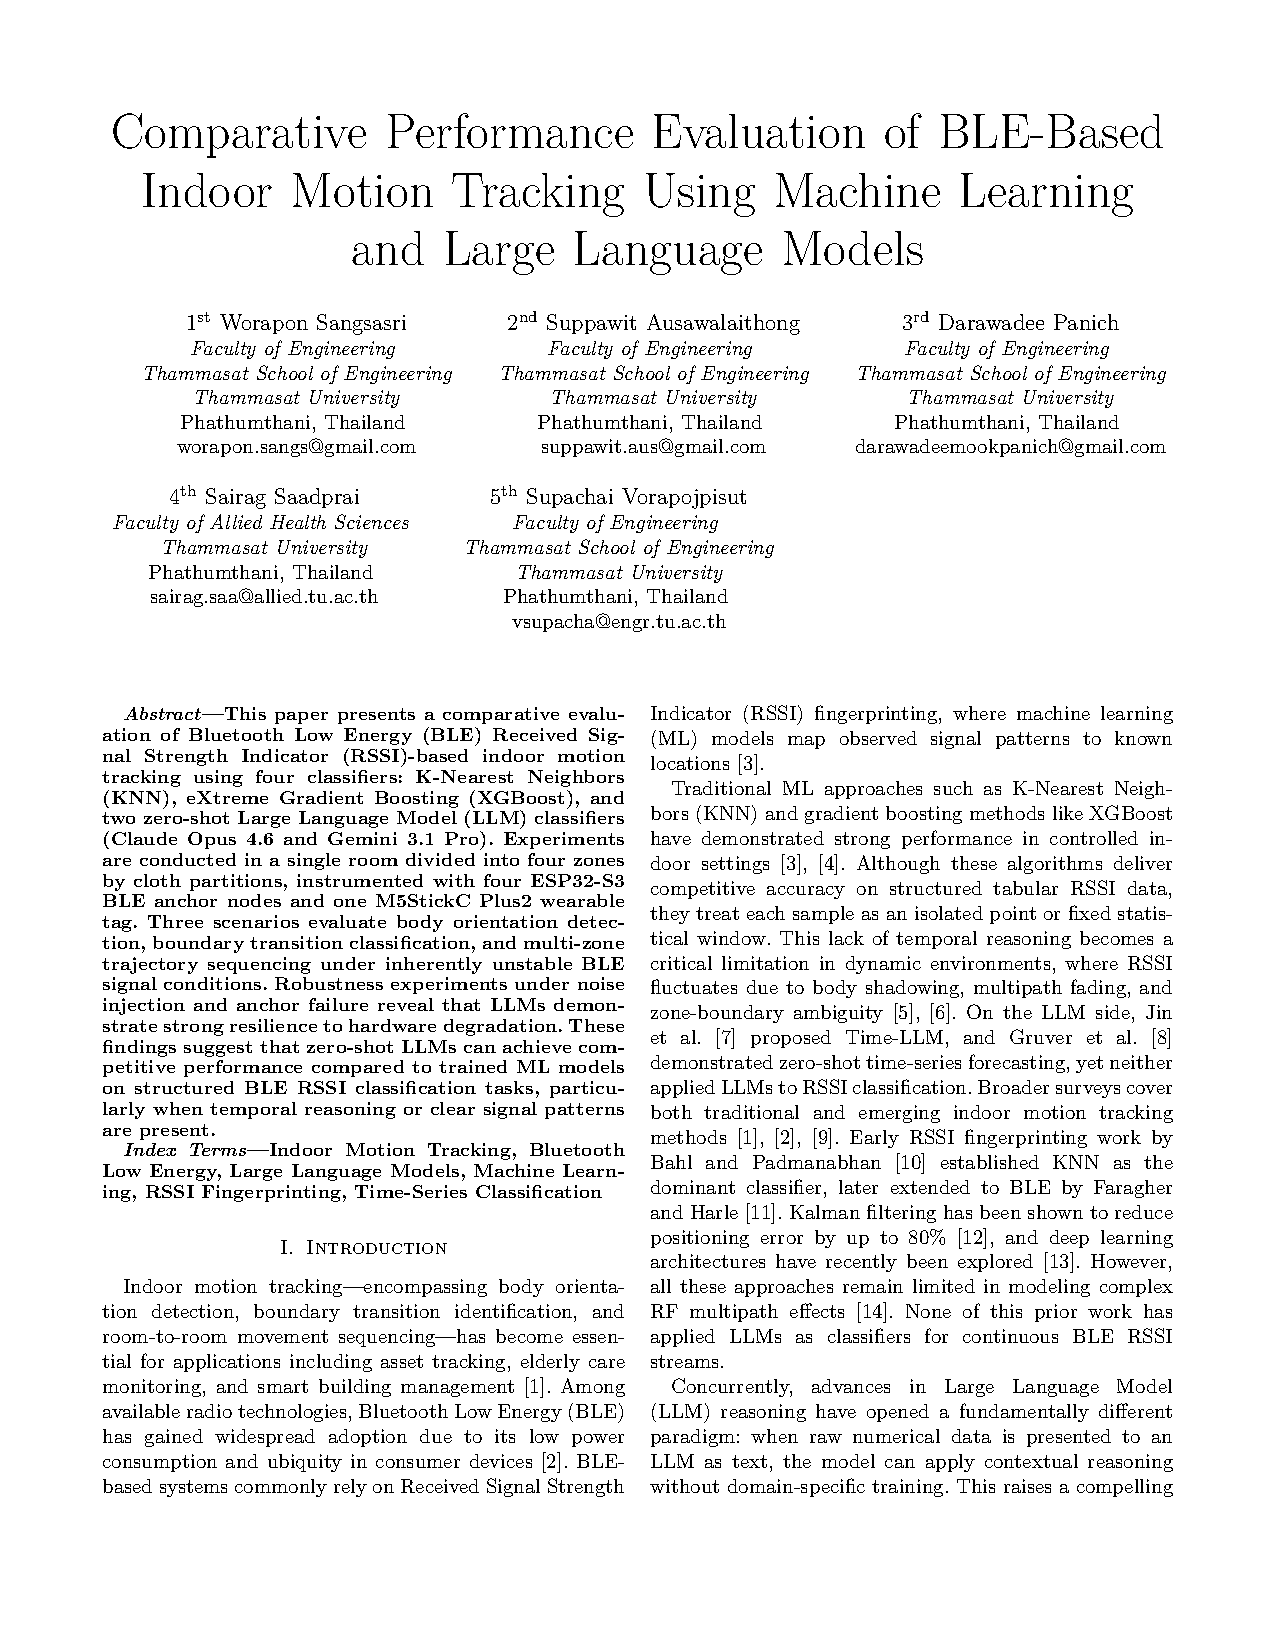
\includepdf[pages=-,pagecommand={}]{assets/appendices/paperieee/Draft_Paper.pdf}
